\documentclass{article} % For LaTeX2e
\usepackage{iclr2021_conference,times}

% Optional math commands from https://github.com/goodfeli/dlbook_notation.
% DO NOT MODIFY THIS COMMENT
% read `https://github.com/James-Yu/LaTeX-Workshop/wiki/Compile#the-root-file`
% read `https://github.com/James-Yu/LaTeX-Workshop/issues/1165`
% !TEX root = iclr2021_conference.tex

%%%%% NEW MATH DEFINITIONS %%%%%

\usepackage{amsmath,amsfonts,bm}

% Mark sections of captions for referring to divisions of figures
\newcommand{\figleft}{{\em (Left)}}
\newcommand{\figcenter}{{\em (Center)}}
\newcommand{\figright}{{\em (Right)}}
\newcommand{\figtop}{{\em (Top)}}
\newcommand{\figbottom}{{\em (Bottom)}}
\newcommand{\captiona}{{\em (a)}}
\newcommand{\captionb}{{\em (b)}}
\newcommand{\captionc}{{\em (c)}}
\newcommand{\captiond}{{\em (d)}}

% Highlight a newly defined term
\newcommand{\newterm}[1]{{\bf #1}}


% Figure reference, lower-case.
\def\figref#1{figure~\ref{#1}}
% Figure reference, capital. For start of sentence
\def\Figref#1{Figure~\ref{#1}}
\def\twofigref#1#2{figures \ref{#1} and \ref{#2}}
\def\quadfigref#1#2#3#4{figures \ref{#1}, \ref{#2}, \ref{#3} and \ref{#4}}
% Section reference, lower-case.
\def\secref#1{section~\ref{#1}}
% Section reference, capital.
\def\Secref#1{Section~\ref{#1}}
% Reference to two sections.
\def\twosecrefs#1#2{sections \ref{#1} and \ref{#2}}
% Reference to three sections.
\def\secrefs#1#2#3{sections \ref{#1}, \ref{#2} and \ref{#3}}
% Reference to an equation, lower-case.
\def\eqref#1{equation~\ref{#1}}
% Reference to an equation, upper case
\def\Eqref#1{Equation~\ref{#1}}
% A raw reference to an equation---avoid using if possible
\def\plaineqref#1{\ref{#1}}
% Reference to a chapter, lower-case.
\def\chapref#1{chapter~\ref{#1}}
% Reference to an equation, upper case.
\def\Chapref#1{Chapter~\ref{#1}}
% Reference to a range of chapters
\def\rangechapref#1#2{chapters\ref{#1}--\ref{#2}}
% Reference to an algorithm, lower-case.
\def\algref#1{algorithm~\ref{#1}}
% Reference to an algorithm, upper case.
\def\Algref#1{Algorithm~\ref{#1}}
\def\twoalgref#1#2{algorithms \ref{#1} and \ref{#2}}
\def\Twoalgref#1#2{Algorithms \ref{#1} and \ref{#2}}
% Reference to a part, lower case
\def\partref#1{part~\ref{#1}}
% Reference to a part, upper case
\def\Partref#1{Part~\ref{#1}}
\def\twopartref#1#2{parts \ref{#1} and \ref{#2}}

\def\ceil#1{\lceil #1 \rceil}
\def\floor#1{\lfloor #1 \rfloor}
\def\1{\bm{1}}
\newcommand{\train}{\mathcal{D}}
\newcommand{\valid}{\mathcal{D_{\mathrm{valid}}}}
\newcommand{\test}{\mathcal{D_{\mathrm{test}}}}

\def\eps{{\epsilon}}


% Random variables
\def\reta{{\textnormal{$\eta$}}}
\def\ra{{\textnormal{a}}}
\def\rb{{\textnormal{b}}}
\def\rc{{\textnormal{c}}}
\def\rd{{\textnormal{d}}}
\def\re{{\textnormal{e}}}
\def\rf{{\textnormal{f}}}
\def\rg{{\textnormal{g}}}
\def\rh{{\textnormal{h}}}
\def\ri{{\textnormal{i}}}
\def\rj{{\textnormal{j}}}
\def\rk{{\textnormal{k}}}
\def\rl{{\textnormal{l}}}
% rm is already a command, just don't name any random variables m
\def\rn{{\textnormal{n}}}
\def\ro{{\textnormal{o}}}
\def\rp{{\textnormal{p}}}
\def\rq{{\textnormal{q}}}
\def\rr{{\textnormal{r}}}
\def\rs{{\textnormal{s}}}
\def\rt{{\textnormal{t}}}
\def\ru{{\textnormal{u}}}
\def\rv{{\textnormal{v}}}
\def\rw{{\textnormal{w}}}
\def\rx{{\textnormal{x}}}
\def\ry{{\textnormal{y}}}
\def\rz{{\textnormal{z}}}

% Random vectors
\def\rvepsilon{{\mathbf{\epsilon}}}
\def\rvtheta{{\mathbf{\theta}}}
\def\rva{{\mathbf{a}}}
\def\rvb{{\mathbf{b}}}
\def\rvc{{\mathbf{c}}}
\def\rvd{{\mathbf{d}}}
\def\rve{{\mathbf{e}}}
\def\rvf{{\mathbf{f}}}
\def\rvg{{\mathbf{g}}}
\def\rvh{{\mathbf{h}}}
\def\rvu{{\mathbf{i}}}
\def\rvj{{\mathbf{j}}}
\def\rvk{{\mathbf{k}}}
\def\rvl{{\mathbf{l}}}
\def\rvm{{\mathbf{m}}}
\def\rvn{{\mathbf{n}}}
\def\rvo{{\mathbf{o}}}
\def\rvp{{\mathbf{p}}}
\def\rvq{{\mathbf{q}}}
\def\rvr{{\mathbf{r}}}
\def\rvs{{\mathbf{s}}}
\def\rvt{{\mathbf{t}}}
\def\rvu{{\mathbf{u}}}
\def\rvv{{\mathbf{v}}}
\def\rvw{{\mathbf{w}}}
\def\rvx{{\mathbf{x}}}
\def\rvy{{\mathbf{y}}}
\def\rvz{{\mathbf{z}}}

% Elements of random vectors
\def\erva{{\textnormal{a}}}
\def\ervb{{\textnormal{b}}}
\def\ervc{{\textnormal{c}}}
\def\ervd{{\textnormal{d}}}
\def\erve{{\textnormal{e}}}
\def\ervf{{\textnormal{f}}}
\def\ervg{{\textnormal{g}}}
\def\ervh{{\textnormal{h}}}
\def\ervi{{\textnormal{i}}}
\def\ervj{{\textnormal{j}}}
\def\ervk{{\textnormal{k}}}
\def\ervl{{\textnormal{l}}}
\def\ervm{{\textnormal{m}}}
\def\ervn{{\textnormal{n}}}
\def\ervo{{\textnormal{o}}}
\def\ervp{{\textnormal{p}}}
\def\ervq{{\textnormal{q}}}
\def\ervr{{\textnormal{r}}}
\def\ervs{{\textnormal{s}}}
\def\ervt{{\textnormal{t}}}
\def\ervu{{\textnormal{u}}}
\def\ervv{{\textnormal{v}}}
\def\ervw{{\textnormal{w}}}
\def\ervx{{\textnormal{x}}}
\def\ervy{{\textnormal{y}}}
\def\ervz{{\textnormal{z}}}

% Random matrices
\def\rmA{{\mathbf{A}}}
\def\rmB{{\mathbf{B}}}
\def\rmC{{\mathbf{C}}}
\def\rmD{{\mathbf{D}}}
\def\rmE{{\mathbf{E}}}
\def\rmF{{\mathbf{F}}}
\def\rmG{{\mathbf{G}}}
\def\rmH{{\mathbf{H}}}
\def\rmI{{\mathbf{I}}}
\def\rmJ{{\mathbf{J}}}
\def\rmK{{\mathbf{K}}}
\def\rmL{{\mathbf{L}}}
\def\rmM{{\mathbf{M}}}
\def\rmN{{\mathbf{N}}}
\def\rmO{{\mathbf{O}}}
\def\rmP{{\mathbf{P}}}
\def\rmQ{{\mathbf{Q}}}
\def\rmR{{\mathbf{R}}}
\def\rmS{{\mathbf{S}}}
\def\rmT{{\mathbf{T}}}
\def\rmU{{\mathbf{U}}}
\def\rmV{{\mathbf{V}}}
\def\rmW{{\mathbf{W}}}
\def\rmX{{\mathbf{X}}}
\def\rmY{{\mathbf{Y}}}
\def\rmZ{{\mathbf{Z}}}

% Elements of random matrices
\def\ermA{{\textnormal{A}}}
\def\ermB{{\textnormal{B}}}
\def\ermC{{\textnormal{C}}}
\def\ermD{{\textnormal{D}}}
\def\ermE{{\textnormal{E}}}
\def\ermF{{\textnormal{F}}}
\def\ermG{{\textnormal{G}}}
\def\ermH{{\textnormal{H}}}
\def\ermI{{\textnormal{I}}}
\def\ermJ{{\textnormal{J}}}
\def\ermK{{\textnormal{K}}}
\def\ermL{{\textnormal{L}}}
\def\ermM{{\textnormal{M}}}
\def\ermN{{\textnormal{N}}}
\def\ermO{{\textnormal{O}}}
\def\ermP{{\textnormal{P}}}
\def\ermQ{{\textnormal{Q}}}
\def\ermR{{\textnormal{R}}}
\def\ermS{{\textnormal{S}}}
\def\ermT{{\textnormal{T}}}
\def\ermU{{\textnormal{U}}}
\def\ermV{{\textnormal{V}}}
\def\ermW{{\textnormal{W}}}
\def\ermX{{\textnormal{X}}}
\def\ermY{{\textnormal{Y}}}
\def\ermZ{{\textnormal{Z}}}

% Vectors
\def\vzero{{\bm{0}}}
\def\vone{{\bm{1}}}
\def\vmu{{\bm{\mu}}}
\def\vtheta{{\bm{\theta}}}
\def\va{{\bm{a}}}
\def\vb{{\bm{b}}}
\def\vc{{\bm{c}}}
\def\vd{{\bm{d}}}
\def\ve{{\bm{e}}}
\def\vf{{\bm{f}}}
\def\vg{{\bm{g}}}
\def\vh{{\bm{h}}}
\def\vi{{\bm{i}}}
\def\vj{{\bm{j}}}
\def\vk{{\bm{k}}}
\def\vl{{\bm{l}}}
\def\vm{{\bm{m}}}
\def\vn{{\bm{n}}}
\def\vo{{\bm{o}}}
\def\vp{{\bm{p}}}
\def\vq{{\bm{q}}}
\def\vr{{\bm{r}}}
\def\vs{{\bm{s}}}
\def\vt{{\bm{t}}}
\def\vu{{\bm{u}}}
\def\vv{{\bm{v}}}
\def\vw{{\bm{w}}}
\def\vx{{\bm{x}}}
\def\vy{{\bm{y}}}
\def\vz{{\bm{z}}}

% Elements of vectors
\def\evalpha{{\alpha}}
\def\evbeta{{\beta}}
\def\evepsilon{{\epsilon}}
\def\evlambda{{\lambda}}
\def\evomega{{\omega}}
\def\evmu{{\mu}}
\def\evpsi{{\psi}}
\def\evsigma{{\sigma}}
\def\evtheta{{\theta}}
\def\eva{{a}}
\def\evb{{b}}
\def\evc{{c}}
\def\evd{{d}}
\def\eve{{e}}
\def\evf{{f}}
\def\evg{{g}}
\def\evh{{h}}
\def\evi{{i}}
\def\evj{{j}}
\def\evk{{k}}
\def\evl{{l}}
\def\evm{{m}}
\def\evn{{n}}
\def\evo{{o}}
\def\evp{{p}}
\def\evq{{q}}
\def\evr{{r}}
\def\evs{{s}}
\def\evt{{t}}
\def\evu{{u}}
\def\evv{{v}}
\def\evw{{w}}
\def\evx{{x}}
\def\evy{{y}}
\def\evz{{z}}

% Matrix
\def\mA{{\bm{A}}}
\def\mB{{\bm{B}}}
\def\mC{{\bm{C}}}
\def\mD{{\bm{D}}}
\def\mE{{\bm{E}}}
\def\mF{{\bm{F}}}
\def\mG{{\bm{G}}}
\def\mH{{\bm{H}}}
\def\mI{{\bm{I}}}
\def\mJ{{\bm{J}}}
\def\mK{{\bm{K}}}
\def\mL{{\bm{L}}}
\def\mM{{\bm{M}}}
\def\mN{{\bm{N}}}
\def\mO{{\bm{O}}}
\def\mP{{\bm{P}}}
\def\mQ{{\bm{Q}}}
\def\mR{{\bm{R}}}
\def\mS{{\bm{S}}}
\def\mT{{\bm{T}}}
\def\mU{{\bm{U}}}
\def\mV{{\bm{V}}}
\def\mW{{\bm{W}}}
\def\mX{{\bm{X}}}
\def\mY{{\bm{Y}}}
\def\mZ{{\bm{Z}}}
\def\mBeta{{\bm{\beta}}}
\def\mPhi{{\bm{\Phi}}}
\def\mLambda{{\bm{\Lambda}}}
\def\mSigma{{\bm{\Sigma}}}

% Tensor
\DeclareMathAlphabet{\mathsfit}{\encodingdefault}{\sfdefault}{m}{sl}
\SetMathAlphabet{\mathsfit}{bold}{\encodingdefault}{\sfdefault}{bx}{n}
\newcommand{\tens}[1]{\bm{\mathsfit{#1}}}
\def\tA{{\tens{A}}}
\def\tB{{\tens{B}}}
\def\tC{{\tens{C}}}
\def\tD{{\tens{D}}}
\def\tE{{\tens{E}}}
\def\tF{{\tens{F}}}
\def\tG{{\tens{G}}}
\def\tH{{\tens{H}}}
\def\tI{{\tens{I}}}
\def\tJ{{\tens{J}}}
\def\tK{{\tens{K}}}
\def\tL{{\tens{L}}}
\def\tM{{\tens{M}}}
\def\tN{{\tens{N}}}
\def\tO{{\tens{O}}}
\def\tP{{\tens{P}}}
\def\tQ{{\tens{Q}}}
\def\tR{{\tens{R}}}
\def\tS{{\tens{S}}}
\def\tT{{\tens{T}}}
\def\tU{{\tens{U}}}
\def\tV{{\tens{V}}}
\def\tW{{\tens{W}}}
\def\tX{{\tens{X}}}
\def\tY{{\tens{Y}}}
\def\tZ{{\tens{Z}}}


% Graph
\def\gA{{\mathcal{A}}}
\def\gB{{\mathcal{B}}}
\def\gC{{\mathcal{C}}}
\def\gD{{\mathcal{D}}}
\def\gE{{\mathcal{E}}}
\def\gF{{\mathcal{F}}}
\def\gG{{\mathcal{G}}}
\def\gH{{\mathcal{H}}}
\def\gI{{\mathcal{I}}}
\def\gJ{{\mathcal{J}}}
\def\gK{{\mathcal{K}}}
\def\gL{{\mathcal{L}}}
\def\gM{{\mathcal{M}}}
\def\gN{{\mathcal{N}}}
\def\gO{{\mathcal{O}}}
\def\gP{{\mathcal{P}}}
\def\gQ{{\mathcal{Q}}}
\def\gR{{\mathcal{R}}}
\def\gS{{\mathcal{S}}}
\def\gT{{\mathcal{T}}}
\def\gU{{\mathcal{U}}}
\def\gV{{\mathcal{V}}}
\def\gW{{\mathcal{W}}}
\def\gX{{\mathcal{X}}}
\def\gY{{\mathcal{Y}}}
\def\gZ{{\mathcal{Z}}}

% Sets
\def\sA{{\mathbb{A}}}
\def\sB{{\mathbb{B}}}
\def\sC{{\mathbb{C}}}
\def\sD{{\mathbb{D}}}
% Don't use a set called E, because this would be the same as our symbol
% for expectation.
\def\sF{{\mathbb{F}}}
\def\sG{{\mathbb{G}}}
\def\sH{{\mathbb{H}}}
\def\sI{{\mathbb{I}}}
\def\sJ{{\mathbb{J}}}
\def\sK{{\mathbb{K}}}
\def\sL{{\mathbb{L}}}
\def\sM{{\mathbb{M}}}
\def\sN{{\mathbb{N}}}
\def\sO{{\mathbb{O}}}
\def\sP{{\mathbb{P}}}
\def\sQ{{\mathbb{Q}}}
\def\sR{{\mathbb{R}}}
\def\sS{{\mathbb{S}}}
\def\sT{{\mathbb{T}}}
\def\sU{{\mathbb{U}}}
\def\sV{{\mathbb{V}}}
\def\sW{{\mathbb{W}}}
\def\sX{{\mathbb{X}}}
\def\sY{{\mathbb{Y}}}
\def\sZ{{\mathbb{Z}}}

% Entries of a matrix
\def\emLambda{{\Lambda}}
\def\emA{{A}}
\def\emB{{B}}
\def\emC{{C}}
\def\emD{{D}}
\def\emE{{E}}
\def\emF{{F}}
\def\emG{{G}}
\def\emH{{H}}
\def\emI{{I}}
\def\emJ{{J}}
\def\emK{{K}}
\def\emL{{L}}
\def\emM{{M}}
\def\emN{{N}}
\def\emO{{O}}
\def\emP{{P}}
\def\emQ{{Q}}
\def\emR{{R}}
\def\emS{{S}}
\def\emT{{T}}
\def\emU{{U}}
\def\emV{{V}}
\def\emW{{W}}
\def\emX{{X}}
\def\emY{{Y}}
\def\emZ{{Z}}
\def\emSigma{{\Sigma}}

% entries of a tensor
% Same font as tensor, without \bm wrapper
\newcommand{\etens}[1]{\mathsfit{#1}}
\def\etLambda{{\etens{\Lambda}}}
\def\etA{{\etens{A}}}
\def\etB{{\etens{B}}}
\def\etC{{\etens{C}}}
\def\etD{{\etens{D}}}
\def\etE{{\etens{E}}}
\def\etF{{\etens{F}}}
\def\etG{{\etens{G}}}
\def\etH{{\etens{H}}}
\def\etI{{\etens{I}}}
\def\etJ{{\etens{J}}}
\def\etK{{\etens{K}}}
\def\etL{{\etens{L}}}
\def\etM{{\etens{M}}}
\def\etN{{\etens{N}}}
\def\etO{{\etens{O}}}
\def\etP{{\etens{P}}}
\def\etQ{{\etens{Q}}}
\def\etR{{\etens{R}}}
\def\etS{{\etens{S}}}
\def\etT{{\etens{T}}}
\def\etU{{\etens{U}}}
\def\etV{{\etens{V}}}
\def\etW{{\etens{W}}}
\def\etX{{\etens{X}}}
\def\etY{{\etens{Y}}}
\def\etZ{{\etens{Z}}}

% The true underlying data generating distribution
\newcommand{\pdata}{p_{\rm{data}}}
% The empirical distribution defined by the training set
\newcommand{\ptrain}{\hat{p}_{\rm{data}}}
\newcommand{\Ptrain}{\hat{P}_{\rm{data}}}
% The model distribution
\newcommand{\pmodel}{p_{\rm{model}}}
\newcommand{\Pmodel}{P_{\rm{model}}}
\newcommand{\ptildemodel}{\tilde{p}_{\rm{model}}}
% Stochastic autoencoder distributions
\newcommand{\pencode}{p_{\rm{encoder}}}
\newcommand{\pdecode}{p_{\rm{decoder}}}
\newcommand{\precons}{p_{\rm{reconstruct}}}

\newcommand{\laplace}{\mathrm{Laplace}} % Laplace distribution

\newcommand{\E}{\mathbb{E}}
\newcommand{\Ls}{\mathcal{L}}
\newcommand{\R}{\mathbb{R}}
\newcommand{\emp}{\tilde{p}}
\newcommand{\lr}{\alpha}
\newcommand{\reg}{\lambda}
\newcommand{\rect}{\mathrm{rectifier}}
\newcommand{\softmax}{\mathrm{softmax}}
\newcommand{\sigmoid}{\sigma}
\newcommand{\softplus}{\zeta}
\newcommand{\KL}{D_{\mathrm{KL}}}
\newcommand{\Var}{\mathrm{Var}}
\newcommand{\standarderror}{\mathrm{SE}}
\newcommand{\Cov}{\mathrm{Cov}}
% Wolfram Mathworld says $L^2$ is for function spaces and $\ell^2$ is for vectors
% But then they seem to use $L^2$ for vectors throughout the site, and so does
% wikipedia.
\newcommand{\normlzero}{L^0}
\newcommand{\normlone}{L^1}
\newcommand{\normltwo}{L^2}
\newcommand{\normlp}{L^p}
\newcommand{\normmax}{L^\infty}

\newcommand{\parents}{Pa} % See usage in notation.tex. Chosen to match Daphne's book.

\DeclareMathOperator*{\argmax}{arg\,max}
\DeclareMathOperator*{\argmin}{arg\,min}

\DeclareMathOperator{\sign}{sign}
\DeclareMathOperator{\Tr}{Tr}
\let\ab\allowbreak


\usepackage{hyperref}
\usepackage{url}

% I got these from this guide:
% https://shantoroy.com/latex/how-to-write-algorithm-in-latex/
% Which I use to highlight how we do the experiment.
\usepackage{algorithm}
\usepackage{arevmath}
\usepackage[noend]{algpseudocode}

\usepackage{graphicx}
\graphicspath{ {.} }


\title{Exploring Neural Network Modularity \\ Using Model Stitching}

% Authors must not appear in the submitted version, you uncomment a line below
% which is labeled "iclrfinalcopy" to anonymize or not.
\author{Adriano Hernandez, Rumen Dangovski \& Peter Y. Lu \thanks{You can find our other work at \url{http://www.a14z.blog/}, \url{http://super-ms.mit.edu/rumen.html}, and \url{https://peterparity.github.io/} respectively.} \\
MIT EECS\\
Cambridge, MA 02139, USA \\
\texttt{\{adrianoh,rumenrd,lup\}@mit.edu}
}

% The \author macro works with any number of authors. There are two commands
% used to separate the names and addresses of multiple authors: \And and \AND.
%
% Using \And between authors leaves it to \LaTeX{} to determine where to break
% the lines. Using \AND forces a linebreak at that point. So, if \LaTeX{}
% puts 3 of 4 authors names on the first line, and the last on the second
% line, try using \AND instead of \And before the third author name.

\newcommand{\fix}{\marginpar{FIX}}
\newcommand{\new}{\marginpar{NEW}}

\iclrfinalcopy % Uncomment for camera-ready version, but NOT for submission.
\begin{document}


\maketitle

\begin{abstract}
We expand \textit{model stitching} (Lenc \& Vedaldi 2015) as a methodology to compare neural networks.
Previously, Bansal, Nakkiran \& Barak used it to compare the representations learned by differently seeded and/or trained neural networks.
We use it to compare the representations learned by neural networks with different architectures.
This gives us insight into the modular structure of neural networks, by helping us map consecutive sequences of layers from one network to those of another.
We think of these sequences of layers as "modules" which may or may not have similar functionality to those of another network.
\end{abstract}


%
%
% Everything below this line
% is the original ICLR template.
% I keep it here specifically for
% the purpose of reminding me of how to do various things...
% I need to figure out how to get citations in there...
% 
% Papers to cite:
% https://arxiv.org/abs/2106.07682 (Revisiting Model Stitching)
%
%
%
%
%%
% https://arxiv.org/abs/2108.01661 (Grounding Representation Similarity with Statistical Testing)
%
% Start here: https://bair.berkeley.edu/blog/2021/11/08/similarity/.
% From this one they basically are trying to create a benchmark to test if a test of similarity is
% good or not. So for example you give them something like CKA or CCA and then they find whether it's
% a good measure or not. However, this "good measure" measure is for A SPECIFIC TASK. So, they are testing
% if FOR A SPECIFIC TASK the measure of similarity is able to discern differences (where accuracy is used
% to tell if the two models are actually different). I'm guessing it's rather harder to use just accuracy
% because it's unclear how you should compare specific layers. They use linear probes (linear classifiers
% trained on top of the intermediate layers we want to compare). They also use accuracy of the whole
% network (though unless you isolate the specific section you change in the network).
%
% Sensitivity: meaningful change is made to a representation => the similarity measure should reflect it.
% Specificity: non-meaningful change is made to a representation => similarity does not change much.
%
% Principle components refers to the principle components as defined by Principle Component Analysis (PCA)
% Read: https://en.wikipedia.org/wiki/Principal_component_analysis. The most informative components
% are the largest ones according to PCA (or at least they can be sorted that way).
%
% It was hard for me to understand what the similarity measures were doing. I need to take a statistics class.
% I also need to review, probably, some aspects of linear algebra or optimization.
%
% I did not totally finish this paper since it was hard to read for me. I will want to write or speak about
% what they are measuring. Here (below) is an outline:
% 1. Definitions of similarity metrics f (OOD and/or linear probe accuracy).
% 2. Definitions of models S (NLP and Vision) and how they were trained
% 3. Descriptions of intuitive tests. We run a test and measure f over it.
%   a. Sensitivity: 
%   b. Specificity: 
% 4. Description of a more rigorous operation
%  a. Definition: pick f (a function from the representation to a real number) as our "accuracy metric"
%  and S as our set of representations to measure similarity. Pick an A inside S (probably the one from the
%  the model with the highest accuracy, or just pick arbitrarily). For all B in S (including cases where
%  A = B) find d(A, B) using the similarity or dissimilarity metric "d" which we are testing, and also find
%  |f(A) - f(B)| which is the variation in "accuracy." Then find Corr(d(A, B), |f(A) - f(B)|) where Corr is
%  a measure of correlation. They use "Tau" and "Rho" which are the Kendall and Spearman measures of
%  correlation, respectively.
%  b. Benchmark 1: layer depth (i.e. which layer).
%  c. Benchmark 2: principle component deletion.
%  d. Pre-training Seed and/or Fine-tuning Seed. For the layer depths the pre-training seed is also varied.
%  For vision the training seed is used (they are Res-Net-14's trained from scratch). For vision no tests seem
%  to be done for PWCCA. I did not read why.
%
% Things that remain to be understood by me:
% 1. The specifics of their experiments (the models, the data, etcetera).
% 2. The definitions of correlation and whether a better "Corr" function might exist.
% 3. The relation between the Wikipedia definitions of "sensitivity" and "specificity" and the usage
%  of those words in the paper (I think it's just meant colloquially, but it's not totally clear).
% 4. The computation and meaning of principle components.
% 5. The meaning and computation of the different similarity metrics. Not only did I not understand them
%  very well, at times I did not even parse them properly.

%%
%% From Revisiting Model Stitching %%
% Understanding intermediate layers using linear classifier probes
% Learning internal representations by error propagation
% Towards understanding learning representations: To what extent do different neural networks learn the same representation, 2018
% Do wide and deep networks learn the same things? uncovering how neural network representations vary with width and depth
% Convergent learning: Do different neural networks learn the same representations?
% Bad global minima exist and sgd can reach them. 
% Insights on representational similarity in neural networks with canonical correlation
% Similarity of neural network representations revisited
% Deep residual learning for image recognition
% Linear mode connectivity and the lottery ticket hypothesis
% On the surprising similarities between supervised and self-supervised models
% Multimodal neurons in artificial neural networks.
%
%

% There is a strict upper limit to 8 pages
% Do NOT refer to the line numbers it automatically generates in your paper
% 
% 
% 
\section{Introduction}
...
\subsection{Motivation}
...
% This will discuss why we are doing this. The main goal is to understand neural networks, but we can think of this
% attempt to understand "modules" as a great boon to transfer learning and cheap computation since it may allow us to
% have the tools necessary to do a lot of iterative tinkering with architectures in an empirical way.

\subsection{Stitching}
...
% This will discuss how stitching works on a high level. It will not introduce any mathematical formalisms or notation.
% Those will probably be used later.

\subsection{Related Approaches}
...
% This will discuss things like CKA, CCA, Procrustes, and stitching without differnet architectures.

\subsection{Preliminary Results}
...
% Here we will analyze our preliminary results and give a high level summary. Currently, my results are disorganized in a bunch
% of .txt log files. I need to get them into figures and tables that are interpretable by us humans (including me).

% Notational notes for myself:
%    %% Stitching %%
% A_{i,j} is the module from i to j inclusive
% A_{\leq N} is the prefix (i.e. module from 0 to N inclusive)
% A_{\geq K} is the suffix of all layers after K.
% AB_{i \rightsquigarrow | \rightarrow \not{\rightarrow} j} is the stitch from A to B from layer i to layer j
%   depeneding on whether the accuracy is unknown, high, or low (so representations are unknown, similar, or differnet)
% To refer to the outputs of networks we use the letter R for representation. For the output of network A
% from layer i we use R_{A, i}. This'd be the input for network A at layer i + 1 or some sort of stitch.
%    %% Mappings %%
% A \rightarrow B
% 
% 
\section{Experimental Setup}
\subsection{Definitions}
We begin with a lot of definitions and then proceed to elucidate the high-level experimental setup
and preliminary results. Our goal from the experiments is to understand what functionality is shared
across pairs of neural network architectures. We rely heavily on a domain-specific language defined
below because it allows us to ascribe terms with precise meaning to all the different types of behaviors
we expect to see.

\subsubsection*{Basic Definitions and Terminology}
\begin{itemize}
   \item Representation: the intermediate output of a neural network, usually refered to as \(R_{A, i}\) if output from layer \(i\) of network \(A\).
   \item Prefix: the first \(N\) layers of a neural network, \(A\). We may call the prefix function \(A_{\leq N}\) or \(A_{<N+1}\) if applicable.
   \item Suffix: the last layers of a neural network \(B\), starting at layer \(K\). We may call the suffix function \(B_{\geq K}\) or \(B_{>K-1}\) if applicable.
   \item Module: a subsequence of consecutive layers in a neural network, similar to the notion of a substring in computer systems. It can also be thought of as a prefix of a suffix, or a suffix of a prefix. It is denoted with the start and ending layers (inclusive). For example \(C_{2,3}\) is the module with layers 2 and 3 of network \(C\). During normal computation, the first layer outputs into it, and it outputs into the fourth layer. Note that single layers are also modules. \(C_{1,1}\) is both the first layer and the first possible module of \(C\). Moreover, prefixes and suffixes are modules.
   \item Submodule: a module inside a module. for example, \(C_{2,2}\) is a submodule of \(C_{2,3}\). This will be used when we wish to describe the internals of modules.
   \item Supermodule: a module within which there is a module. This will be used when we wish to group modules.
   \item Sender: when a module recieves input from a previous module we call that previous module the sender. We may also say that a module is \emph{sending} when we wish to express that it is the sender.
   \item Reciever: The module some other module is sending to. We may also say that it is \emph{recieving}.
   \item Expected sender (or reciever): absent of stitching, the module that would be the sender or the reciever to/from the current module.
   \item Expected input (or output): the output of the expected sender or reciever during normal computation.
\end{itemize}

\subsubsection*{Stitching}
We define stitching in the same way as Bansal et. al. 
Say we wish to stitch two networks \(A\) and \(B\).
We will calculate the output of a prefix of \(A\),
input it into our stitch \(S\), and then input the output
of \(S\) into a suffix of \(B\). Say we take the
output of \(A\) at layer \(i\), input it into \(S\),
and then take the output of \(S\) and input it into
\(B\) at layer \(j+1\). We say that layer \(i\) of
\(A\) was stitched \emph{into} layer \(j+1\) of \(B\).
The composition \(S \circ A_{\leq i}\) has replaced
the expected sender, \(B_{\leq j}\) of \(B_{>j}\).
As discussed by Bansal et. al, this enables us to compare
the representations \(R_{A,i}\) and \(R_{B,j}\).

The stitch \(S\) is a function whose domain is the set of possible \(R_{A,i}\)
and whose range is in the same space as \(R_{B,j}\). For the same reasons as Bansal et. al.
we use simple function classes like 1x1 convolutions where applicable and strided convolutions
elsewhere.

The network formed with \(B_{\geq j+1} \circ S \circ A_{\leq i}\) is called the 
\emph{stitched network} and is often denoted as \(AB_{i \rightsquigarrow j+1}\). The stitched 
network is frozen in all layers except for \(S\), which is trained with gradient descent
so as to approximate the best possible choice for \(S\). If the resulting accuracy
is high then we refer to the stitched network as \(AB_{i \rightarrow j+1}\) and we say
that \(A\) is \emph{stitchable} to \(B\) through those layers: \(\exists AB_{i \rightarrow j+1}\).
If the resulting accuracy is low, we refer to the stitched network as \(AB_{i \not{\rightarrow} j+1}\)
and we say that \(A\) is not stitchable to \(B\) through those layers.

\subsubsection*{Representational Mappings}
A representational mapping between neural networks \(A\) of length and \(B\) is a mapping that assigns
at most one \(R_{B,j}\) for every \(R_{A,i}\). We sometimes use the layer indices \(i\) and \(j\)
as shorthand.

We establish the mapping as follows: for each valid \(i\) in \(A\), find the \(j\) in \(B\)
such that \(R_{A,i}\) is most similar to \(R_{B,j}\) out of all possible \(j\) and
\(\exists AB_{i \rightarrow j+1}\). We refer to the mapping as \(A \rightarrow B\). There are
other ways to define such a relation, but we pick this one for simplicity.
Intuitively this says that those two representations are, to an extent, interchangeable.
We also hope that this mapping will be injective and monotonic.
By monotonic we simply mean that if \(i_{1} < i_{2}\), \(i_{1}\) maps to \(j_{1}\),
and \(i_{2}\) maps to \(j_{2}\), then it should be the case that \(j_{1} < j_{2}\). This simply
means that the network is learning more abstract notions as data flows through it.

The precise reader will note that while the representations may be interchangeable in one direction
they may not be in both, depending on the type of stitch. That is to say,  \(\exists AB_{i \rightarrow j+1}\)
does not imply \(\exists BA_{j \rightarrow i+1}\), even with linear transformations and 1x1 convolutions
because of the possibility of drastic changes in dimensionality. We use \(\rightarrow\) and \(\leftarrow\)
or flip the order of the operands to differentiate the two directions.
When we wish to express \(\exists AB_{i \rightarrow j+1} \land \exists BA_{j \rightarrow i+1}\),
we may often say \(AB_{i \leftrightarrow j}\). We may also define a two-way representational mapping,
\(A \leftrightarrow B = (A \rightarrow B) \cap (B \rightarrow A)\), though it is not a mapping
in the mathematical sense, but instead a list of tuples.
% Begin Footnote
\footnote{For a set of tuples \(C\), Define the reverse tuple set \(V(C) = \{(b, a) \forall (a, b) \in C\}\).
For a mapping \(f: D \to R\) we define its set of tuples, \(T(f) = \{(x, f(x)) \forall x \in D\}\).
For \(f: D \to R, g: R \to D\), we define \(f \cap g = T(f) \cap V(T(g))\). We can also define
\(f \cup g = T(f) \cup V(T(g))\). Note that \(f \cap g\) is always a subset of \(D x R\), and
that \(f \cap g = V(g \cap f)\)}.
% End Footnote

The precise reader will also note that high accuracy should be relative to some baseline. We define what is high
experimentally and using random (untrained) networks. When stitching different architectures we compare the accuracy
with that of the \emph{least accurate} architecture that went into the stitch. That means that if we stitch from
a very large (or wide) network to a very small one, or vice versa, we should expect the smaller network to be a
bottleneck on accuracy.

\subsubsection*{Modular Mapping}
Using our representational mappings, we establish a more general notion of modular mappings based on modules. A Modular mapping
tells us about what modules in two different neural networks might have shared functionality based on representational similarity.
Intuitively, if one module is mapped to another, then the latter can be swapped out for the former, with two stitches, in the latter's network.
Informally, for two networks \(A\) and \(B\), \(A_{i_1, i_2}\) is mapped to \(B_{j_1, j_2}\) if we can find a pair of stitches \(S_1, S_2\), such that the accuracy is high for
\(B_{>j_2} \circ S_2 \circ A_{i_1,i_2} \circ S_1 \circ B_{<j_1}\). Since it's possible to infer this from \(A \rightarrow B\) and \(B \rightarrow A\),
however, we infer it from \(\exists BA_{j_1 \rightarrow i_1}\) and \(\exists AB_{i_2 \rightarrow j_2+1}\).

To find these modular mappings we can simply brute force for all possible indices, \(i_1, i_2, j_1, j_2\),
given our pre-computed representational mappings. If we denote the length (in layers) of \(A\) as \(N_1\) and
that of \(B\) as \(N_2\), The runtime of the brute force algorithm is \(\mathcal{O}(\alpha N_1 N_2)\) where \(\alpha\) is
the worst-case time necessary to optimize a stitch between any pair of layers.

However, we would prefer to also try and enforce monotonicity of the modular mapping. If two modules, \(M_1 = A_{i_1, i_2}, M_2 = A_{i_3, i_4}\),
have the property that \(i_2 < i_3\), we say that \(M_1 < M_2\). Monotonicity means that of we have any two modules in \(A\),
\(M_{A_1}, M_{A_2}\), and any two modules in \(B\), \(M_{B_1}, M_{B_2}\), such that \(M_{A_1} \Rightarrow M_{B_1}\)
and \(M_{A_2} \Rightarrow M_{B_2}\), then \(M_{A_1} < M_{A_2}\)implies \(M_{B_1} < M_{B_2}\). Monotonicity is preferable, because
it makes the mapping more interpretable. It may not be the case that the modular mapping is monotonic, but we can instead choose to
focus on a subset of module pairs that is. We present an algorithm below which given two neural networks finds a monotonic subset of
\(A \Rightarrow B\).

\begin{center}
\begin{algorithm}
\caption{Find A Monotonic Modular Mapping Subset}
\begin{algorithmic}[h]
\Procedure{MFind(\(A\), \(B\))}{}
      \State Pretrain and Freeze \(A\) and \(B\) seperately
      \State \(A\) has length \(N\)
      \State \(B\) has length \(M\)
      \State Find \(A\rightarrow B\) through brute force
      \State Find \(B\rightarrow A\) through brute force
      \State \(i_{start} = 1\)
      \State \(j_{start} = 1\)
      \State Initialize \(MM = \{\}\)
      \For{\(i_{end} \in [1, N-1]\)}
         \For{\(j_{end} \in [j_{start}, M-1]\)}
            \If{\((B_{j_{start}-1} \rightarrow A_{i_{start}}) \land (A_{i_{end}} \rightarrow B_{j_{end}+1})\)}
               \State Add \((A_{i_{start}, i_{end}}, B_{j_{start}, j_{end}})\) to \(MM\)
               \State \(i_{start} = i_{end} + 1\)
               \State \(j_{start} = j_{end} + 1\)
               \State Break Inner Loop
            \EndIf
         \EndFor
      \EndFor
      \State Return \(MM\)
\EndProcedure
\end{algorithmic}
\end{algorithm}
\end{center}

\subsection{Hypotheses}
Now that we know how to talk about modules, we introduce 4 main idealized cases that may present themselves when we
try to modularly map two different neural networks of different sizes. We assume that these mappings are all monotonic.
We describe these assuming that the sender network is at most as long as the reciever network.

\begin{itemize}
   \item Layer to layer (L2L) mapping: single layers (in shorter networks) may have the same functionality as single layers in longer networks. Additional layers in longer networks introduce new functionality. This mapping is injective, but not necessarily surjective.
   \item Layer to module (L2M) mapping: single layers (in shorter networks) may have the same functionality as modules in longer networks. The long networks have the same functionality, but better. This mapping is injective and ideally surjective.
   \item Module to module (M2M) mapping: modules (in shorter networks) may have the same functionality as modules in longer networks. This mapping is injective and ideally surjective.
   \item No (N) mapping: informally, when there is M2M mapping, but the modules are so big as to be uninformative.
\end{itemize}

It is possible that our mappings will not be monotonic, but we hope to find that they are. It is an elegant
simplifiying assumption.

Given this assumption, it is (only) possible to have these four cases outlined above. However, which one
is most prevalent at a specific segment of a network may change: we may start with L2L mappings followed by
M2M or N mappings, for example. To define a notion of this, we introduce \textit{realms}. Realms are pairs
of supermodules within which submodules obey a single mapping mode (L2L, L2M, M2M, or N).
More generally, if within a pair of supermodules behavior follows some pattern, we label it a realm.

Thus, we may re-pharse our goal as that of describing the realms of modular mappings for different
neural network architectures. To do this we generate a monotonic modular mapping based on representational
mappings which we found using stitching. This helps us understand for pairs of networks, where they have the
same functionality in a precise way.

\subsection{Networks and Dataset}
We focused on varying only the random seed of the neural network. To simplify our analysis we also used the CIFAR-10 dataset
with standard resnets. These currently only include ResNet18, but will soon also include  ResNet34, ResNet50, ResNet101, ResNet152.
The optimizers and hyperparameters used are further elucidated in the appendix.

For layers with the same width and height we used 1x1 convolutions as our stitching function class. For layers with different dimensions
we utilized the fact that the dimensions of the layers are powers of two (in our networks). In stitches that required downsampling (due
to smaller dimensions in the reciever) we used strided convolutions. In stitches that required upsampling we simply used a nearest
upsampling followed by a 1x1 convolution (which you can think of as reversed strided convolutions).

\subsection{Tests and Controls}
\subsubsection*{Networks of the same architecture}
First we stitched networks of each architecture with other networks of the same architecture. We trained lists of networks for each 
architecture. For each list we called the first element the \textit{pivot}. The pivot was stitched to each of the other networks
in the same list, including itself. For every pair of networks we stitched each layer in the sender network to each layer in the
reciever network. 

For the purpose of creating a control, we made sure that there was a random (untrained) reciever network in the list. We also swapped 
pivots with another untrained network which was stitched with all the other networks in the list. This ensured that we had baselines
for resulting accuracy (and therefore similarity).

You can think of the result of each pair of networks' stitches as a square matrix of accuracies, where the row denotes the layer of the
sender network and the column denotes the layer of the reciever network. The accuracy at that elements is our measure of representational
similarity. These tables are tiled into a tensor which represents the results of the stitch. In the depth dimension we average to find
the average similarity over all our experiments for that architecture. Note that we insert zero at layer pairs that are not stichable
due to dissimilar shapes.

\subsubsection*{Networks of different architectures}
We will conduct the same experiment as above, but where the pivot (sender) architecture is different from the reciever architecture.
For each pair of architectures, we pick a pivot of each architecture along with a (small) list of recievers of the other architecture.
We then repeated the procedure from the case with two identical architectures. Note that instead of a square matrix of accuracies, we
have a rectangular matrix of accuracies. This matrix will be tall if the sender network is longer than the reciever network, and wide
in the other case.

\subsection{Testing Algorithm}
More details will be elucidated in the appendix.

\section{Results}
\subsection{Summary}
We have preliminary results that suggest the expected: networks of the same architecture yield a high similarity
along the layer-to-layer matrix diagonal, with decreasing accuracies towards the top right and bottom left corners. This tells us
that they are in a L2L realm (where corresponding layers have similar output representations and therefore functionality).
For a random network, we have random behavior. We trained on a ResNet18 and have graphics below.
\begin{center}
   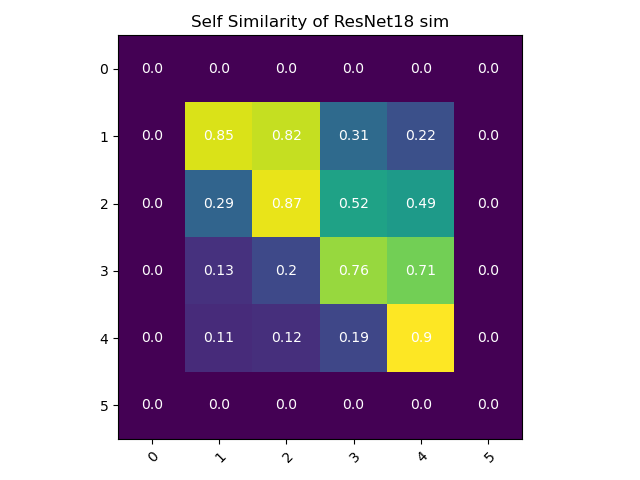
\includegraphics[width=6.5cm]{sim.png}
   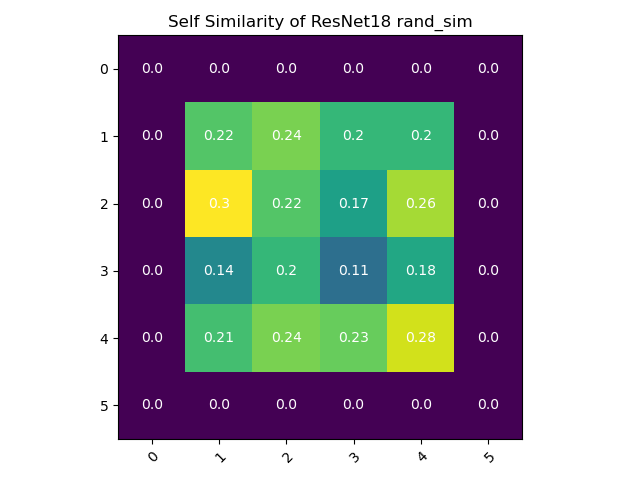
\includegraphics[width=6.5cm]{rand.png}
\end{center}
\subsection{Figures}
...

% Figures that make sense when they are in black and white are ideal
% \begin{figure}[h]
% \begin{center}
% %\framebox[4.0in]{$\;$}
% \fbox{\rule[-.5cm]{0cm}{4cm} \rule[-.5cm]{4cm}{0cm}}
% \end{center}
% \caption{Sample figure caption.}
% \end{figure}

\subsection{Tables}
...

% \begin{table}[h]
% \caption{Sample table title}
% \label{sample-table}
% \begin{center}
% \begin{tabular}{ll}
% \multicolumn{1}{c}{\bf PART}  &\multicolumn{1}{c}{\bf DESCRIPTION}
% \\ \hline \\
% Dendrite         &Input terminal \\
% Axon             &Output terminal \\
% Soma             &Cell body (contains cell nucleus) \\
% \end{tabular}
% \end{center}
% \end{table}

\section{Analysis and Interpretation of Results}
\subsection{Interpretation}
...
% It didn't work.

\subsection{Significance}
...
% What this means for the future and the field.

\section{Conclusions}
...
% We'll write our conclusions in a nice format here.

\section*{Acknowledgments}
Thank you to the SuperUROP benefactors (MIT EECS) for funding this project.

\bibliography{iclr2021_conference}
\bibliographystyle{iclr2021_conference}

\appendix
\section{Appendix}
...

\end{document}
